% Options for packages loaded elsewhere
\PassOptionsToPackage{unicode}{hyperref}
\PassOptionsToPackage{hyphens}{url}
%
\documentclass[
]{article}
\usepackage{amsmath,amssymb}
\usepackage{iftex}
\ifPDFTeX
  \usepackage[T1]{fontenc}
  \usepackage[utf8]{inputenc}
  \usepackage{textcomp} % provide euro and other symbols
\else % if luatex or xetex
  \usepackage{unicode-math} % this also loads fontspec
  \defaultfontfeatures{Scale=MatchLowercase}
  \defaultfontfeatures[\rmfamily]{Ligatures=TeX,Scale=1}
\fi
\usepackage{lmodern}
\ifPDFTeX\else
  % xetex/luatex font selection
\fi
% Use upquote if available, for straight quotes in verbatim environments
\IfFileExists{upquote.sty}{\usepackage{upquote}}{}
\IfFileExists{microtype.sty}{% use microtype if available
  \usepackage[]{microtype}
  \UseMicrotypeSet[protrusion]{basicmath} % disable protrusion for tt fonts
}{}
\makeatletter
\@ifundefined{KOMAClassName}{% if non-KOMA class
  \IfFileExists{parskip.sty}{%
    \usepackage{parskip}
  }{% else
    \setlength{\parindent}{0pt}
    \setlength{\parskip}{6pt plus 2pt minus 1pt}}
}{% if KOMA class
  \KOMAoptions{parskip=half}}
\makeatother
\usepackage{xcolor}
\usepackage[margin=1in]{geometry}
\usepackage{color}
\usepackage{fancyvrb}
\newcommand{\VerbBar}{|}
\newcommand{\VERB}{\Verb[commandchars=\\\{\}]}
\DefineVerbatimEnvironment{Highlighting}{Verbatim}{commandchars=\\\{\}}
% Add ',fontsize=\small' for more characters per line
\usepackage{framed}
\definecolor{shadecolor}{RGB}{248,248,248}
\newenvironment{Shaded}{\begin{snugshade}}{\end{snugshade}}
\newcommand{\AlertTok}[1]{\textcolor[rgb]{0.94,0.16,0.16}{#1}}
\newcommand{\AnnotationTok}[1]{\textcolor[rgb]{0.56,0.35,0.01}{\textbf{\textit{#1}}}}
\newcommand{\AttributeTok}[1]{\textcolor[rgb]{0.13,0.29,0.53}{#1}}
\newcommand{\BaseNTok}[1]{\textcolor[rgb]{0.00,0.00,0.81}{#1}}
\newcommand{\BuiltInTok}[1]{#1}
\newcommand{\CharTok}[1]{\textcolor[rgb]{0.31,0.60,0.02}{#1}}
\newcommand{\CommentTok}[1]{\textcolor[rgb]{0.56,0.35,0.01}{\textit{#1}}}
\newcommand{\CommentVarTok}[1]{\textcolor[rgb]{0.56,0.35,0.01}{\textbf{\textit{#1}}}}
\newcommand{\ConstantTok}[1]{\textcolor[rgb]{0.56,0.35,0.01}{#1}}
\newcommand{\ControlFlowTok}[1]{\textcolor[rgb]{0.13,0.29,0.53}{\textbf{#1}}}
\newcommand{\DataTypeTok}[1]{\textcolor[rgb]{0.13,0.29,0.53}{#1}}
\newcommand{\DecValTok}[1]{\textcolor[rgb]{0.00,0.00,0.81}{#1}}
\newcommand{\DocumentationTok}[1]{\textcolor[rgb]{0.56,0.35,0.01}{\textbf{\textit{#1}}}}
\newcommand{\ErrorTok}[1]{\textcolor[rgb]{0.64,0.00,0.00}{\textbf{#1}}}
\newcommand{\ExtensionTok}[1]{#1}
\newcommand{\FloatTok}[1]{\textcolor[rgb]{0.00,0.00,0.81}{#1}}
\newcommand{\FunctionTok}[1]{\textcolor[rgb]{0.13,0.29,0.53}{\textbf{#1}}}
\newcommand{\ImportTok}[1]{#1}
\newcommand{\InformationTok}[1]{\textcolor[rgb]{0.56,0.35,0.01}{\textbf{\textit{#1}}}}
\newcommand{\KeywordTok}[1]{\textcolor[rgb]{0.13,0.29,0.53}{\textbf{#1}}}
\newcommand{\NormalTok}[1]{#1}
\newcommand{\OperatorTok}[1]{\textcolor[rgb]{0.81,0.36,0.00}{\textbf{#1}}}
\newcommand{\OtherTok}[1]{\textcolor[rgb]{0.56,0.35,0.01}{#1}}
\newcommand{\PreprocessorTok}[1]{\textcolor[rgb]{0.56,0.35,0.01}{\textit{#1}}}
\newcommand{\RegionMarkerTok}[1]{#1}
\newcommand{\SpecialCharTok}[1]{\textcolor[rgb]{0.81,0.36,0.00}{\textbf{#1}}}
\newcommand{\SpecialStringTok}[1]{\textcolor[rgb]{0.31,0.60,0.02}{#1}}
\newcommand{\StringTok}[1]{\textcolor[rgb]{0.31,0.60,0.02}{#1}}
\newcommand{\VariableTok}[1]{\textcolor[rgb]{0.00,0.00,0.00}{#1}}
\newcommand{\VerbatimStringTok}[1]{\textcolor[rgb]{0.31,0.60,0.02}{#1}}
\newcommand{\WarningTok}[1]{\textcolor[rgb]{0.56,0.35,0.01}{\textbf{\textit{#1}}}}
\usepackage{graphicx}
\makeatletter
\def\maxwidth{\ifdim\Gin@nat@width>\linewidth\linewidth\else\Gin@nat@width\fi}
\def\maxheight{\ifdim\Gin@nat@height>\textheight\textheight\else\Gin@nat@height\fi}
\makeatother
% Scale images if necessary, so that they will not overflow the page
% margins by default, and it is still possible to overwrite the defaults
% using explicit options in \includegraphics[width, height, ...]{}
\setkeys{Gin}{width=\maxwidth,height=\maxheight,keepaspectratio}
% Set default figure placement to htbp
\makeatletter
\def\fps@figure{htbp}
\makeatother
\setlength{\emergencystretch}{3em} % prevent overfull lines
\providecommand{\tightlist}{%
  \setlength{\itemsep}{0pt}\setlength{\parskip}{0pt}}
\setcounter{secnumdepth}{-\maxdimen} % remove section numbering
\ifLuaTeX
  \usepackage{selnolig}  % disable illegal ligatures
\fi
\usepackage{bookmark}
\IfFileExists{xurl.sty}{\usepackage{xurl}}{} % add URL line breaks if available
\urlstyle{same}
\hypersetup{
  pdftitle={TDDE15-Lab 4},
  pdfauthor={Fredrik Ramberg},
  hidelinks,
  pdfcreator={LaTeX via pandoc}}

\title{TDDE15-Lab 4}
\author{Fredrik Ramberg}
\date{}

\begin{document}
\maketitle

\section{Part 2.1}\label{part-2.1}

\textbf{Imports}

\begin{Shaded}
\begin{Highlighting}[]
\FunctionTok{library}\NormalTok{(}\StringTok{"mvtnorm"}\NormalTok{)}
\end{Highlighting}
\end{Shaded}

\textbf{2.1. Implementing GP Regression.}

This first exercise will have you writing your own code for the Gaussian
process regression model: y = f (x) + \emph{Epsilon} with \emph{Epsilon}
∼ N (0, σ2 n) and f ∼ GP(0, k(x, x′))

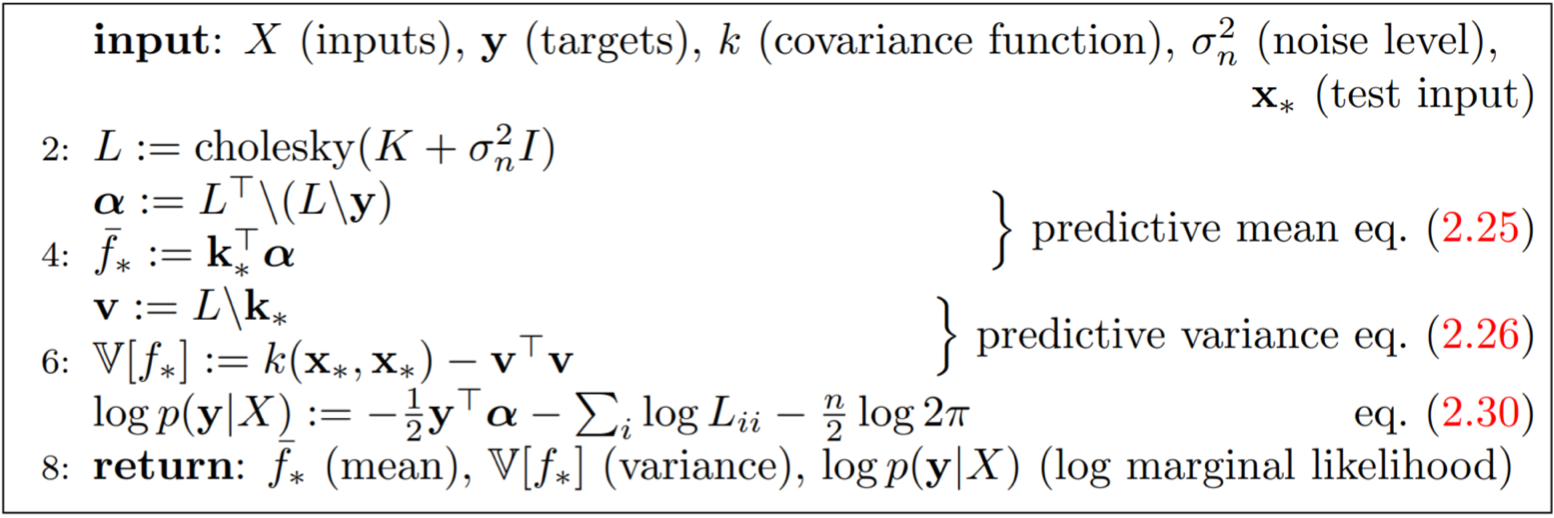
\includegraphics[width=5.54167in,height=\textheight]{images/Screenshot 2024-10-13 at 15.21.25.png}

\begin{Shaded}
\begin{Highlighting}[]
\CommentTok{\# Covariance function}
\NormalTok{SquaredExpKernel }\OtherTok{\textless{}{-}} \ControlFlowTok{function}\NormalTok{(x1,x2,}\AttributeTok{sigmaF=}\DecValTok{1}\NormalTok{,}\AttributeTok{l=}\DecValTok{3}\NormalTok{)\{}
\NormalTok{  n1 }\OtherTok{\textless{}{-}} \FunctionTok{length}\NormalTok{(x1)}
\NormalTok{  n2 }\OtherTok{\textless{}{-}} \FunctionTok{length}\NormalTok{(x2)}
\NormalTok{  K }\OtherTok{\textless{}{-}} \FunctionTok{matrix}\NormalTok{(}\ConstantTok{NA}\NormalTok{,n1,n2)}
  \ControlFlowTok{for}\NormalTok{ (i }\ControlFlowTok{in} \DecValTok{1}\SpecialCharTok{:}\NormalTok{n2)\{}
\NormalTok{    K[,i] }\OtherTok{\textless{}{-}}\NormalTok{ sigmaF}\SpecialCharTok{\^{}}\DecValTok{2}\SpecialCharTok{*}\FunctionTok{exp}\NormalTok{(}\SpecialCharTok{{-}}\FloatTok{0.5}\SpecialCharTok{*}\NormalTok{( (x1}\SpecialCharTok{{-}}\NormalTok{x2[i])}\SpecialCharTok{/}\NormalTok{l)}\SpecialCharTok{\^{}}\DecValTok{2}\NormalTok{ )}
\NormalTok{  \}}
  \FunctionTok{return}\NormalTok{(K)}
\NormalTok{\}}

\NormalTok{posteriorGP }\OtherTok{\textless{}{-}} \ControlFlowTok{function}\NormalTok{(X, y, XStar, sigmaNoise, k, ...)\{}
\NormalTok{  n }\OtherTok{\textless{}{-}} \FunctionTok{length}\NormalTok{(X)}
\NormalTok{  K }\OtherTok{\textless{}{-}} \FunctionTok{k}\NormalTok{(X, X, ...)}
\NormalTok{  kStar }\OtherTok{\textless{}{-}} \FunctionTok{k}\NormalTok{(X,XStar, ...)}
  
  \CommentTok{\#Cholesky }
\NormalTok{  L }\OtherTok{\textless{}{-}} \FunctionTok{t}\NormalTok{(}\FunctionTok{chol}\NormalTok{(K }\SpecialCharTok{+}\NormalTok{ sigmaNoise}\SpecialCharTok{\^{}}\DecValTok{2}\SpecialCharTok{*}\FunctionTok{diag}\NormalTok{(n)))}

  \CommentTok{\#alpha}
\NormalTok{  alpha }\OtherTok{\textless{}{-}} \FunctionTok{solve}\NormalTok{(}\FunctionTok{t}\NormalTok{(L),}\FunctionTok{solve}\NormalTok{(L,y))}
  
  \CommentTok{\#Posterior mean = fStar}
\NormalTok{  kStar }\OtherTok{\textless{}{-}} \FunctionTok{k}\NormalTok{(X, XStar, ...)}
\NormalTok{  fStar }\OtherTok{\textless{}{-}} \FunctionTok{t}\NormalTok{(kStar)}\SpecialCharTok{\%*\%}\NormalTok{alpha}

  \CommentTok{\#Posterior variance}
\NormalTok{  v }\OtherTok{\textless{}{-}} \FunctionTok{solve}\NormalTok{(L,kStar)}
\NormalTok{  variance }\OtherTok{\textless{}{-}} \FunctionTok{k}\NormalTok{(XStar, XStar, ...) }\SpecialCharTok{{-}} \FunctionTok{t}\NormalTok{(v)}\SpecialCharTok{\%*\%}\NormalTok{v}
  
  \FunctionTok{return}\NormalTok{(}\FunctionTok{list}\NormalTok{(}\AttributeTok{mean =}\NormalTok{fStar, }\AttributeTok{variance =}\NormalTok{variance))}
\NormalTok{\}}
\end{Highlighting}
\end{Shaded}

\begin{Shaded}
\begin{Highlighting}[]
\CommentTok{\#Hyperparameters}
\NormalTok{sigmaF }\OtherTok{\textless{}{-}} \DecValTok{1}
\NormalTok{l }\OtherTok{\textless{}{-}} \FloatTok{0.3}
\NormalTok{sigmaNoise }\OtherTok{\textless{}{-}} \FloatTok{0.1}


\CommentTok{\#observation}
\NormalTok{obs }\OtherTok{\textless{}{-}} \FunctionTok{data.frame}\NormalTok{(}\AttributeTok{X =} \FloatTok{0.4}\NormalTok{, }\AttributeTok{Y =} \FloatTok{0.719}\NormalTok{)}

\CommentTok{\#test points}
\NormalTok{XStar }\OtherTok{\textless{}{-}} \FunctionTok{seq}\NormalTok{(}\SpecialCharTok{{-}}\DecValTok{1}\NormalTok{,}\DecValTok{1}\NormalTok{,}\AttributeTok{length=}\DecValTok{100}\NormalTok{)}

\NormalTok{posterior }\OtherTok{\textless{}{-}} \FunctionTok{posteriorGP}\NormalTok{(obs}\SpecialCharTok{$}\NormalTok{X, obs}\SpecialCharTok{$}\NormalTok{Y, XStar, sigmaNoise, SquaredExpKernel, sigmaF, l)}

\CommentTok{\# mean and posterior}
\NormalTok{posterior\_mean }\OtherTok{\textless{}{-}}\NormalTok{ posterior}\SpecialCharTok{$}\NormalTok{mean}
\NormalTok{posterior\_variance }\OtherTok{\textless{}{-}} \FunctionTok{diag}\NormalTok{(posterior}\SpecialCharTok{$}\NormalTok{variance)}

\CommentTok{\# 95\% confidence intervals}
\NormalTok{upper\_bound }\OtherTok{\textless{}{-}}\NormalTok{ posterior\_mean }\SpecialCharTok{+} \FloatTok{1.96} \SpecialCharTok{*} \FunctionTok{sqrt}\NormalTok{(posterior\_variance)}
\NormalTok{lower\_bound }\OtherTok{\textless{}{-}}\NormalTok{ posterior\_mean }\SpecialCharTok{{-}} \FloatTok{1.96} \SpecialCharTok{*} \FunctionTok{sqrt}\NormalTok{(posterior\_variance)}

\CommentTok{\# Plot posterior mean and 95\% confidence intervals}
\FunctionTok{plot}\NormalTok{(XStar, posterior\_mean, }\AttributeTok{type =} \StringTok{"l"}\NormalTok{, }\AttributeTok{col =} \StringTok{"blue"}\NormalTok{, }\AttributeTok{lwd =} \DecValTok{2}\NormalTok{,}
     \AttributeTok{ylim =} \FunctionTok{c}\NormalTok{(}\FunctionTok{min}\NormalTok{(lower\_bound), }\FunctionTok{max}\NormalTok{(upper\_bound)),}
     \AttributeTok{xlab =} \StringTok{"x"}\NormalTok{, }\AttributeTok{ylab =} \StringTok{"f(x)"}\NormalTok{, }\AttributeTok{main =} \StringTok{"Posterior Mean and 95\% Confidence Bands of Single Observation"}\NormalTok{)}
\FunctionTok{lines}\NormalTok{(XStar, upper\_bound, }\AttributeTok{col =} \StringTok{"red"}\NormalTok{, }\AttributeTok{lty =} \DecValTok{2}\NormalTok{)}
\FunctionTok{lines}\NormalTok{(XStar, lower\_bound, }\AttributeTok{col =} \StringTok{"red"}\NormalTok{, }\AttributeTok{lty =} \DecValTok{2}\NormalTok{)}
\FunctionTok{points}\NormalTok{(obs}\SpecialCharTok{$}\NormalTok{X, obs}\SpecialCharTok{$}\NormalTok{Y, }\AttributeTok{col =} \StringTok{"black"}\NormalTok{, }\AttributeTok{pch =} \DecValTok{19}\NormalTok{)  }\CommentTok{\# Plot the training point}
\end{Highlighting}
\end{Shaded}

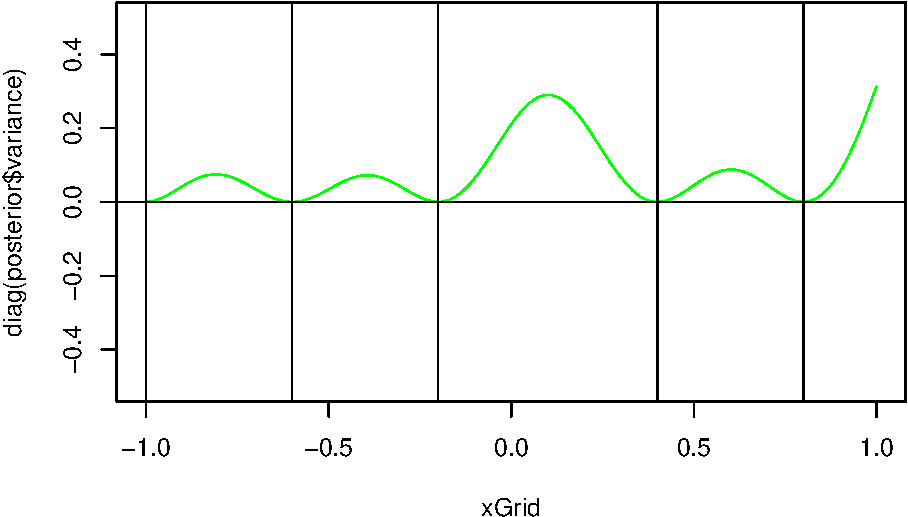
\includegraphics{lab4_files/figure-latex/unnamed-chunk-3-1.pdf}

\textbf{(3)} Update your posterior from (2) with another observation:
(x,y) = (−0.6,−0.044). Plot the posterior mean of f over the interval x
∈ {[}−1, 1{]}. Plot also 95 \% probability (point-wise) bands for f.

\textbf{Hint}: Updating the posterior after one observation with a new
observation gives the same result as updating the prior directly with
the two observations.

\begin{Shaded}
\begin{Highlighting}[]
\NormalTok{obs2 }\OtherTok{\textless{}{-}} \FunctionTok{rbind}\NormalTok{(obs, }\FunctionTok{data.frame}\NormalTok{(}\AttributeTok{X=} \SpecialCharTok{{-}}\FloatTok{0.6}\NormalTok{, }\AttributeTok{Y =} \SpecialCharTok{{-}}\FloatTok{0.044}\NormalTok{))}

\NormalTok{posterior }\OtherTok{\textless{}{-}} \FunctionTok{posteriorGP}\NormalTok{(obs2}\SpecialCharTok{$}\NormalTok{X, obs2}\SpecialCharTok{$}\NormalTok{Y, XStar, sigmaNoise, SquaredExpKernel, sigmaF, l)}

\CommentTok{\# mean and posterior}
\NormalTok{posterior\_mean }\OtherTok{\textless{}{-}}\NormalTok{ posterior}\SpecialCharTok{$}\NormalTok{mean}
\NormalTok{posterior\_variance }\OtherTok{\textless{}{-}} \FunctionTok{diag}\NormalTok{(posterior}\SpecialCharTok{$}\NormalTok{variance)}

\CommentTok{\# 95\% confidence intervals}
\NormalTok{upper\_bound }\OtherTok{\textless{}{-}}\NormalTok{ posterior\_mean }\SpecialCharTok{+} \FloatTok{1.96} \SpecialCharTok{*} \FunctionTok{sqrt}\NormalTok{(posterior\_variance)}
\NormalTok{lower\_bound }\OtherTok{\textless{}{-}}\NormalTok{ posterior\_mean }\SpecialCharTok{{-}} \FloatTok{1.96} \SpecialCharTok{*} \FunctionTok{sqrt}\NormalTok{(posterior\_variance)}

\CommentTok{\# Plot posterior mean and 95\% confidence intervals}
\FunctionTok{plot}\NormalTok{(XStar, posterior\_mean, }\AttributeTok{type =} \StringTok{"l"}\NormalTok{, }\AttributeTok{col =} \StringTok{"blue"}\NormalTok{, }\AttributeTok{lwd =} \DecValTok{2}\NormalTok{,}
     \AttributeTok{ylim =} \FunctionTok{c}\NormalTok{(}\FunctionTok{min}\NormalTok{(lower\_bound), }\FunctionTok{max}\NormalTok{(upper\_bound)),}
     \AttributeTok{xlab =} \StringTok{"x"}\NormalTok{, }\AttributeTok{ylab =} \StringTok{"f(x)"}\NormalTok{, }\AttributeTok{main =} \StringTok{"Posterior Mean and 95\% Confidence Bands of Two Observations"}\NormalTok{)}
\FunctionTok{lines}\NormalTok{(XStar, upper\_bound, }\AttributeTok{col =} \StringTok{"red"}\NormalTok{, }\AttributeTok{lty =} \DecValTok{2}\NormalTok{)}
\FunctionTok{lines}\NormalTok{(XStar, lower\_bound, }\AttributeTok{col =} \StringTok{"red"}\NormalTok{, }\AttributeTok{lty =} \DecValTok{2}\NormalTok{)}
\FunctionTok{points}\NormalTok{(obs2}\SpecialCharTok{$}\NormalTok{X, obs2}\SpecialCharTok{$}\NormalTok{Y, }\AttributeTok{col =} \StringTok{"black"}\NormalTok{, }\AttributeTok{pch =} \DecValTok{19}\NormalTok{)  }\CommentTok{\# Plot the training point}
\end{Highlighting}
\end{Shaded}

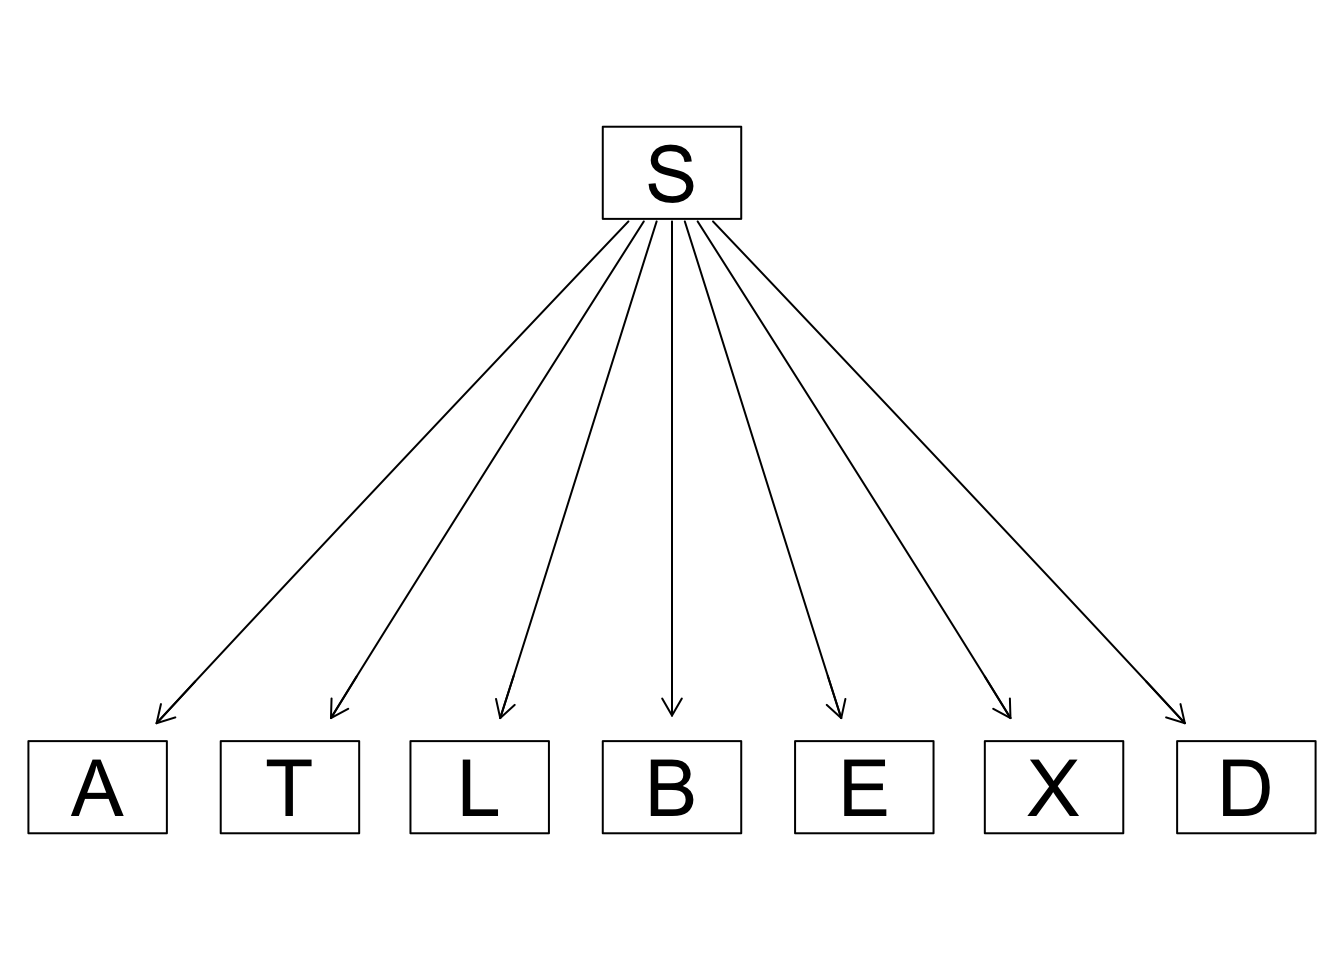
\includegraphics{lab4_files/figure-latex/unnamed-chunk-4-1.pdf}

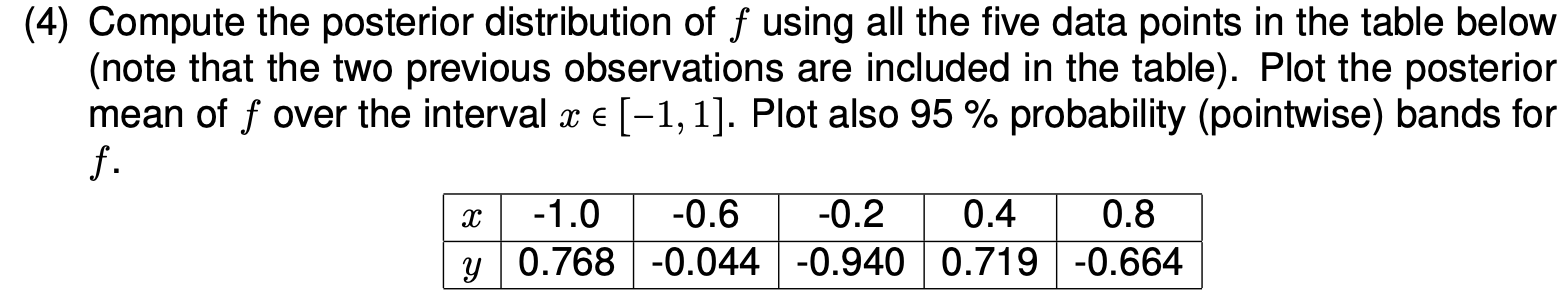
\includegraphics{images/Screenshot 2024-10-13 at 16.21.55.png}

\begin{Shaded}
\begin{Highlighting}[]
\NormalTok{obs5 }\OtherTok{\textless{}{-}} \FunctionTok{data.frame}\NormalTok{(}\AttributeTok{X =} \FunctionTok{c}\NormalTok{(}\SpecialCharTok{{-}}\DecValTok{1}\NormalTok{,}\SpecialCharTok{{-}}\FloatTok{0.6}\NormalTok{,}\SpecialCharTok{{-}}\FloatTok{0.2}\NormalTok{,}\FloatTok{0.4}\NormalTok{,}\FloatTok{0.8}\NormalTok{), }
                   \AttributeTok{Y =} \FunctionTok{c}\NormalTok{(}\FloatTok{0.768}\NormalTok{,}\SpecialCharTok{{-}}\FloatTok{0.044}\NormalTok{,}\SpecialCharTok{{-}}\FloatTok{0.940}\NormalTok{,}\FloatTok{0.719}\NormalTok{,}\SpecialCharTok{{-}}\FloatTok{0.664}\NormalTok{))}

\NormalTok{posterior }\OtherTok{\textless{}{-}} \FunctionTok{posteriorGP}\NormalTok{(obs5}\SpecialCharTok{$}\NormalTok{X, obs5}\SpecialCharTok{$}\NormalTok{Y, XStar, sigmaNoise, SquaredExpKernel, sigmaF, l)}

\CommentTok{\# mean and posterior}
\NormalTok{posterior\_mean }\OtherTok{\textless{}{-}}\NormalTok{ posterior}\SpecialCharTok{$}\NormalTok{mean}
\NormalTok{posterior\_variance }\OtherTok{\textless{}{-}} \FunctionTok{diag}\NormalTok{(posterior}\SpecialCharTok{$}\NormalTok{variance)}

\CommentTok{\# 95\% confidence intervals}
\NormalTok{upper\_bound }\OtherTok{\textless{}{-}}\NormalTok{ posterior\_mean }\SpecialCharTok{+} \FloatTok{1.96} \SpecialCharTok{*} \FunctionTok{sqrt}\NormalTok{(posterior\_variance)}
\NormalTok{lower\_bound }\OtherTok{\textless{}{-}}\NormalTok{ posterior\_mean }\SpecialCharTok{{-}} \FloatTok{1.96} \SpecialCharTok{*} \FunctionTok{sqrt}\NormalTok{(posterior\_variance)}

\CommentTok{\# Plot posterior mean and 95\% confidence intervals}
\FunctionTok{plot}\NormalTok{(XStar, posterior\_mean, }\AttributeTok{type =} \StringTok{"l"}\NormalTok{, }\AttributeTok{col =} \StringTok{"blue"}\NormalTok{, }\AttributeTok{lwd =} \DecValTok{2}\NormalTok{,}
     \AttributeTok{ylim =} \FunctionTok{c}\NormalTok{(}\FunctionTok{min}\NormalTok{(lower\_bound), }\FunctionTok{max}\NormalTok{(upper\_bound)),}
     \AttributeTok{xlab =} \StringTok{"x"}\NormalTok{, }\AttributeTok{ylab =} \StringTok{"f(x)"}\NormalTok{, }\AttributeTok{main =} \StringTok{"Posterior Mean and 95\% Confidence Bands of Five Observations"}\NormalTok{)}
\FunctionTok{lines}\NormalTok{(XStar, upper\_bound, }\AttributeTok{col =} \StringTok{"red"}\NormalTok{, }\AttributeTok{lty =} \DecValTok{2}\NormalTok{)}
\FunctionTok{lines}\NormalTok{(XStar, lower\_bound, }\AttributeTok{col =} \StringTok{"red"}\NormalTok{, }\AttributeTok{lty =} \DecValTok{2}\NormalTok{)}
\FunctionTok{points}\NormalTok{(obs5}\SpecialCharTok{$}\NormalTok{X, obs5}\SpecialCharTok{$}\NormalTok{Y, }\AttributeTok{col =} \StringTok{"black"}\NormalTok{, }\AttributeTok{pch =} \DecValTok{19}\NormalTok{)  }\CommentTok{\# Plot the training point}
\end{Highlighting}
\end{Shaded}

\includegraphics{lab4_files/figure-latex/unnamed-chunk-5-1.pdf}

\textbf{(5)} Repeat (4), this time with hyperparameters σf = 1 and l =
1. Compare the results.

\begin{Shaded}
\begin{Highlighting}[]
\CommentTok{\#changing the hyperparameters, the rest is the same .....}

\NormalTok{posterior }\OtherTok{\textless{}{-}} \FunctionTok{posteriorGP}\NormalTok{(obs5}\SpecialCharTok{$}\NormalTok{X, obs5}\SpecialCharTok{$}\NormalTok{Y, XStar, sigmaNoise, SquaredExpKernel, }\AttributeTok{sigmaF =} \DecValTok{1}\NormalTok{, }\AttributeTok{l =} \DecValTok{1}\NormalTok{)}

\CommentTok{\# mean and posterior}
\NormalTok{posterior\_mean }\OtherTok{\textless{}{-}}\NormalTok{ posterior}\SpecialCharTok{$}\NormalTok{mean}
\NormalTok{posterior\_variance }\OtherTok{\textless{}{-}} \FunctionTok{diag}\NormalTok{(posterior}\SpecialCharTok{$}\NormalTok{variance)}

\CommentTok{\# 95\% confidence intervals}
\NormalTok{upper\_bound }\OtherTok{\textless{}{-}}\NormalTok{ posterior\_mean }\SpecialCharTok{+} \FloatTok{1.96} \SpecialCharTok{*} \FunctionTok{sqrt}\NormalTok{(posterior\_variance)}
\NormalTok{lower\_bound }\OtherTok{\textless{}{-}}\NormalTok{ posterior\_mean }\SpecialCharTok{{-}} \FloatTok{1.96} \SpecialCharTok{*} \FunctionTok{sqrt}\NormalTok{(posterior\_variance)}

\CommentTok{\# Plot posterior mean and 95\% confidence intervals}
\FunctionTok{plot}\NormalTok{(XStar, posterior\_mean, }\AttributeTok{type =} \StringTok{"l"}\NormalTok{, }\AttributeTok{col =} \StringTok{"blue"}\NormalTok{, }\AttributeTok{lwd =} \DecValTok{2}\NormalTok{,}
     \AttributeTok{ylim =} \FunctionTok{c}\NormalTok{(}\FunctionTok{min}\NormalTok{(lower\_bound), }\FunctionTok{max}\NormalTok{(upper\_bound)),}
     \AttributeTok{xlab =} \StringTok{"x"}\NormalTok{, }\AttributeTok{ylab =} \StringTok{"f(x)"}\NormalTok{, }\AttributeTok{main =} \StringTok{"Posterior Mean and 95\% Confidence Bands of Two Observations"}\NormalTok{)}
\FunctionTok{lines}\NormalTok{(XStar, upper\_bound, }\AttributeTok{col =} \StringTok{"red"}\NormalTok{, }\AttributeTok{lty =} \DecValTok{2}\NormalTok{)}
\FunctionTok{lines}\NormalTok{(XStar, lower\_bound, }\AttributeTok{col =} \StringTok{"red"}\NormalTok{, }\AttributeTok{lty =} \DecValTok{2}\NormalTok{)}
\FunctionTok{points}\NormalTok{(obs5}\SpecialCharTok{$}\NormalTok{X, obs5}\SpecialCharTok{$}\NormalTok{Y, }\AttributeTok{col =} \StringTok{"black"}\NormalTok{, }\AttributeTok{pch =} \DecValTok{19}\NormalTok{)  }\CommentTok{\# Plot the training point}
\end{Highlighting}
\end{Shaded}

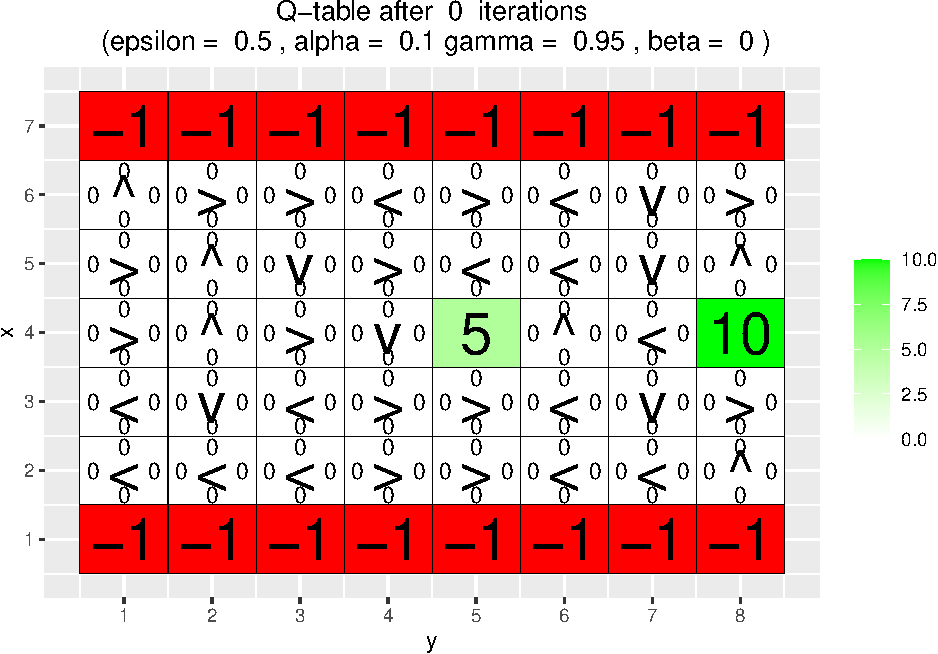
\includegraphics{lab4_files/figure-latex/unnamed-chunk-6-1.pdf}

\section{\texorpdfstring{\textbf{Part 2.2}}{Part 2.2}}\label{part-2.2}

\textbf{Imports and data structure}

\begin{Shaded}
\begin{Highlighting}[]
\FunctionTok{library}\NormalTok{(kernlab)}

\NormalTok{tempData }\OtherTok{\textless{}{-}} \FunctionTok{read.csv}\NormalTok{(}\StringTok{"https://github.com/STIMALiU/AdvMLCourse/raw/master/GaussianProcess/Code/TempTullinge.csv"}\NormalTok{, }\AttributeTok{header=}\ConstantTok{TRUE}\NormalTok{, }\AttributeTok{sep=}\StringTok{";"}\NormalTok{)}
\NormalTok{tempData }\OtherTok{\textless{}{-}} \FunctionTok{cbind}\NormalTok{(tempData, }\AttributeTok{time =} \DecValTok{1}\SpecialCharTok{:}\FunctionTok{nrow}\NormalTok{(tempData))}
\NormalTok{tempData }\OtherTok{\textless{}{-}} \FunctionTok{cbind}\NormalTok{(tempData, }\AttributeTok{day =}\NormalTok{ ((tempData}\SpecialCharTok{$}\NormalTok{time}\DecValTok{{-}1}\NormalTok{)}\SpecialCharTok{\%\%}\DecValTok{365}\NormalTok{)}\SpecialCharTok{+}\DecValTok{1}\NormalTok{)}

\NormalTok{trainData }\OtherTok{\textless{}{-}} \FunctionTok{subset}\NormalTok{(tempData, (time }\SpecialCharTok{{-}} \DecValTok{1}\NormalTok{)}\SpecialCharTok{\%\%}\DecValTok{5} \SpecialCharTok{==} \DecValTok{0}\NormalTok{)}
\end{Highlighting}
\end{Shaded}

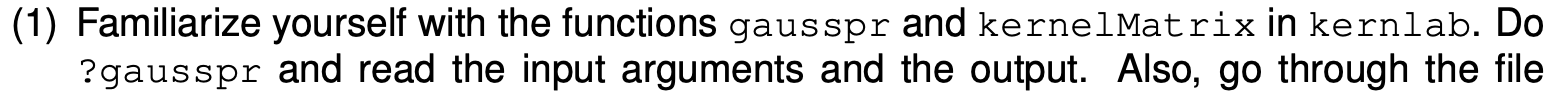
\includegraphics{images/Screenshot 2024-10-13 at 17.14.24.png}

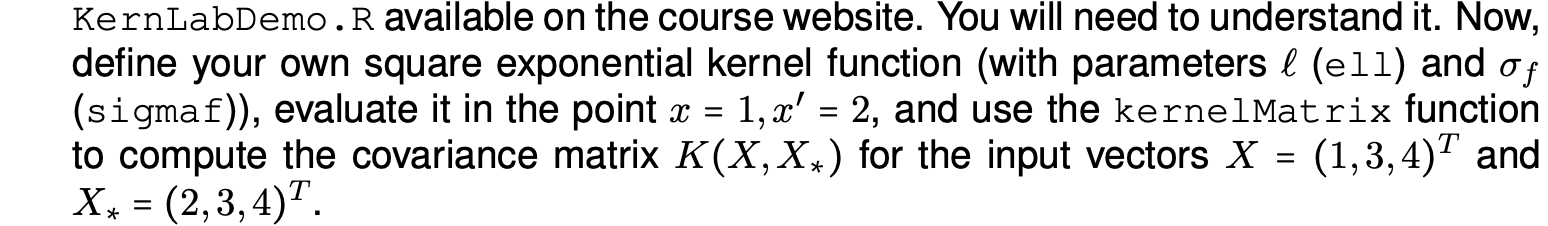
\includegraphics{images/Screenshot 2024-10-13 at 17.14.46.png}

\begin{Shaded}
\begin{Highlighting}[]
\CommentTok{\#nested Square Exponetial Kernel}
\NormalTok{nestedSEK }\OtherTok{\textless{}{-}} \ControlFlowTok{function}\NormalTok{(}\AttributeTok{sigmaF=}\DecValTok{1}\NormalTok{,}\AttributeTok{l=}\DecValTok{3}\NormalTok{) \{}
\NormalTok{  fixedSEK }\OtherTok{\textless{}{-}} \ControlFlowTok{function}\NormalTok{(x1,x2)\{}
\NormalTok{    n1 }\OtherTok{\textless{}{-}} \FunctionTok{length}\NormalTok{(x1)}
\NormalTok{    n2 }\OtherTok{\textless{}{-}} \FunctionTok{length}\NormalTok{(x2)}
\NormalTok{    K }\OtherTok{\textless{}{-}} \FunctionTok{matrix}\NormalTok{(}\ConstantTok{NA}\NormalTok{,n1,n2)}
    \ControlFlowTok{for}\NormalTok{ (i }\ControlFlowTok{in} \DecValTok{1}\SpecialCharTok{:}\NormalTok{n2)\{}
\NormalTok{      K[,i] }\OtherTok{\textless{}{-}}\NormalTok{ sigmaF}\SpecialCharTok{\^{}}\DecValTok{2}\SpecialCharTok{*}\FunctionTok{exp}\NormalTok{(}\SpecialCharTok{{-}}\FloatTok{0.5}\SpecialCharTok{*}\NormalTok{( (x1}\SpecialCharTok{{-}}\NormalTok{x2[i])}\SpecialCharTok{/}\NormalTok{l)}\SpecialCharTok{\^{}}\DecValTok{2}\NormalTok{ )}
\NormalTok{    \}}
    \FunctionTok{return}\NormalTok{(K)}
\NormalTok{  \}}
  \FunctionTok{class}\NormalTok{(fixedSEK) }\OtherTok{\textless{}{-}} \StringTok{\textquotesingle{}kernel\textquotesingle{}}
  \FunctionTok{return}\NormalTok{(fixedSEK)}
\NormalTok{\}}

\NormalTok{SEK }\OtherTok{\textless{}{-}} \FunctionTok{nestedSEK}\NormalTok{()}

\CommentTok{\#testing kernal function for x=1, xstar=2}
\FunctionTok{SEK}\NormalTok{(}\DecValTok{1}\NormalTok{,}\DecValTok{2}\NormalTok{)}
\end{Highlighting}
\end{Shaded}

\begin{verbatim}
##           [,1]
## [1,] 0.9459595
\end{verbatim}

\begin{Shaded}
\begin{Highlighting}[]
\CommentTok{\# kernel matrix where x = X, y = Xstar}
\FunctionTok{kernelMatrix}\NormalTok{(}\AttributeTok{kernel =}\NormalTok{ SEK, }\AttributeTok{x =} \FunctionTok{c}\NormalTok{(}\DecValTok{1}\NormalTok{,}\DecValTok{3}\NormalTok{,}\DecValTok{4}\NormalTok{), }\AttributeTok{y =}\FunctionTok{c}\NormalTok{(}\DecValTok{2}\NormalTok{,}\DecValTok{3}\NormalTok{,}\DecValTok{4}\NormalTok{))}
\end{Highlighting}
\end{Shaded}

\begin{verbatim}
## An object of class "kernelMatrix"
##           [,1]      [,2]      [,3]
## [1,] 0.9459595 0.8007374 0.6065307
## [2,] 0.9459595 1.0000000 0.9459595
## [3,] 0.8007374 0.9459595 1.0000000
\end{verbatim}

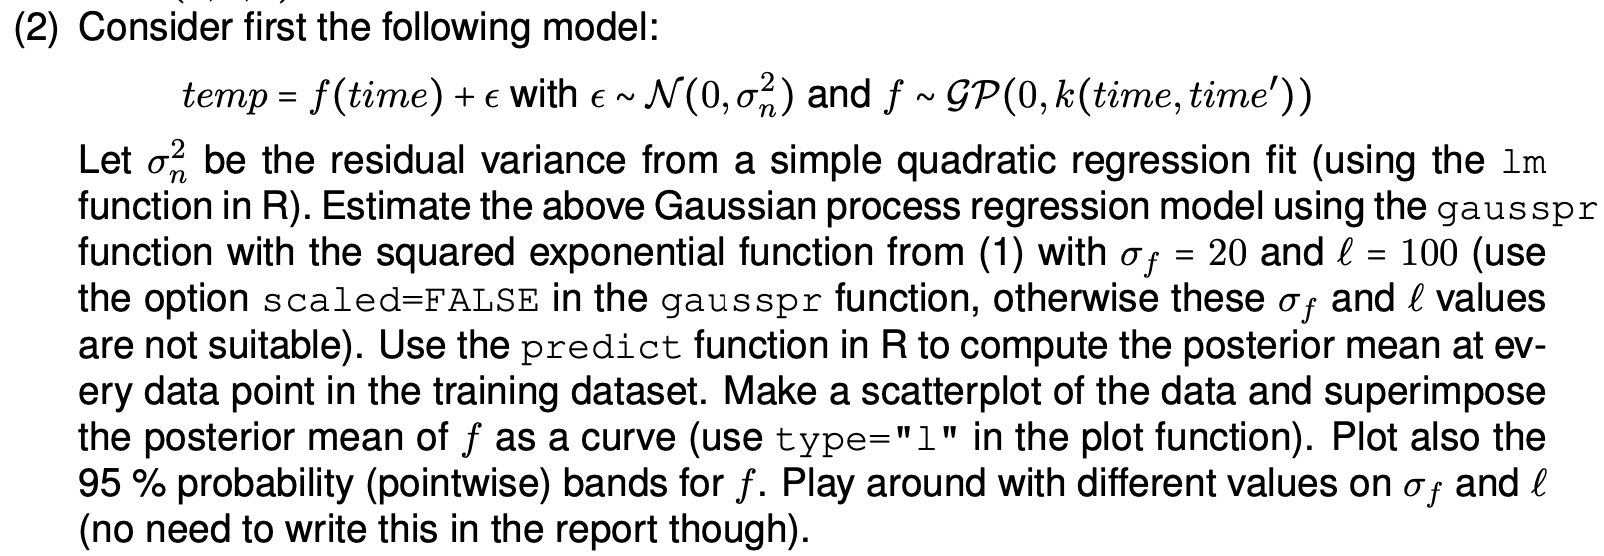
\includegraphics{images/Screenshot 2024-10-13 at 17.13.16.png}

\begin{Shaded}
\begin{Highlighting}[]
\CommentTok{\#Estimating sigmaNoise from fitting a two degree polynomial to data}
\NormalTok{polyFit }\OtherTok{\textless{}{-}} \FunctionTok{lm}\NormalTok{(trainData}\SpecialCharTok{$}\NormalTok{temp }\SpecialCharTok{\textasciitilde{}}\NormalTok{  trainData}\SpecialCharTok{$}\NormalTok{time }\SpecialCharTok{+} \FunctionTok{I}\NormalTok{(trainData}\SpecialCharTok{$}\NormalTok{time}\SpecialCharTok{\^{}}\DecValTok{2}\NormalTok{))}
\NormalTok{sigmaNoise }\OtherTok{\textless{}{-}} \FunctionTok{sd}\NormalTok{(polyFit}\SpecialCharTok{$}\NormalTok{residuals)}

\CommentTok{\#setting hyperparameters in kernel function}
\NormalTok{SEK }\OtherTok{\textless{}{-}} \FunctionTok{nestedSEK}\NormalTok{(}\AttributeTok{sigmaF =} \DecValTok{20}\NormalTok{, }\AttributeTok{l =} \DecValTok{100}\NormalTok{)}

\NormalTok{modelGP }\OtherTok{\textless{}{-}} \FunctionTok{gausspr}\NormalTok{(trainData}\SpecialCharTok{$}\NormalTok{time, trainData}\SpecialCharTok{$}\NormalTok{temp, }\AttributeTok{scaled =} \ConstantTok{FALSE}\NormalTok{, }\AttributeTok{kernel =}\NormalTok{ SEK, }\AttributeTok{var =}\NormalTok{ sigmaNoise}\SpecialCharTok{\^{}}\DecValTok{2}\NormalTok{)}

\NormalTok{posteriorMeanTime }\OtherTok{\textless{}{-}} \FunctionTok{predict}\NormalTok{(modelGP)}


\FunctionTok{plot}\NormalTok{(}\AttributeTok{x=}\NormalTok{ trainData}\SpecialCharTok{$}\NormalTok{time, }\AttributeTok{y =}\NormalTok{ trainData}\SpecialCharTok{$}\NormalTok{temp,}
     \AttributeTok{xlab =} \StringTok{"time"}\NormalTok{, }\AttributeTok{ylab =} \StringTok{"temp"}\NormalTok{, }\AttributeTok{main =} \StringTok{"Temperature predictions"}\NormalTok{, }\AttributeTok{lwd =} \FloatTok{1.5}\NormalTok{)}
\FunctionTok{lines}\NormalTok{(}\AttributeTok{x=}\NormalTok{trainData}\SpecialCharTok{$}\NormalTok{time, }\AttributeTok{y =}\NormalTok{ posteriorMeanTime, }\AttributeTok{col =} \StringTok{"red"}\NormalTok{, }\AttributeTok{lwd =} \DecValTok{3}\NormalTok{)}
\FunctionTok{legend}\NormalTok{(}\StringTok{"bottomright"}\NormalTok{, }\AttributeTok{legend=}\FunctionTok{c}\NormalTok{(}\StringTok{"Data"}\NormalTok{, }\StringTok{"Predictions"}\NormalTok{), }\AttributeTok{pch=}\FunctionTok{c}\NormalTok{(}\DecValTok{1}\NormalTok{, }\ConstantTok{NA}\NormalTok{), }\AttributeTok{lty=}\FunctionTok{c}\NormalTok{(}\ConstantTok{NA}\NormalTok{, }\DecValTok{1}\NormalTok{), }\AttributeTok{lwd=}\FunctionTok{c}\NormalTok{(}\ConstantTok{NA}\NormalTok{, }\DecValTok{2}\NormalTok{), }\AttributeTok{col=}\FunctionTok{c}\NormalTok{(}\StringTok{"black"}\NormalTok{, }\StringTok{"red"}\NormalTok{))}
\end{Highlighting}
\end{Shaded}

\includegraphics{lab4_files/figure-latex/unnamed-chunk-9-1.pdf}

\hfill\break
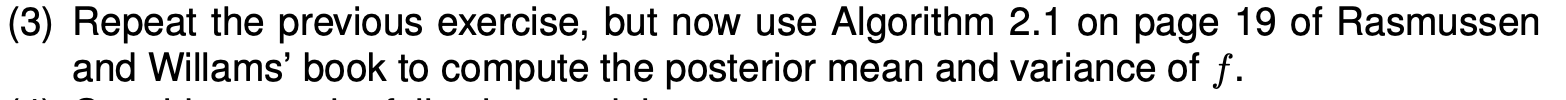
\includegraphics{images/Screenshot 2024-10-13 at 18.21.20.png}

\begin{Shaded}
\begin{Highlighting}[]
\CommentTok{\#setting hyperparameters in kernel function}
\NormalTok{SEK }\OtherTok{\textless{}{-}} \FunctionTok{nestedSEK}\NormalTok{(}\AttributeTok{sigmaF =} \DecValTok{20}\NormalTok{, }\AttributeTok{l =} \DecValTok{100}\NormalTok{)}

\CommentTok{\#modelGP \textless{}{-} gausspr(trainData$time, trainData$temp, scaled = FALSE, kernel = SEK, var = sigmaNoise\^{}2)}


\NormalTok{posterior }\OtherTok{\textless{}{-}} \FunctionTok{posteriorGP}\NormalTok{(trainData}\SpecialCharTok{$}\NormalTok{time, trainData}\SpecialCharTok{$}\NormalTok{temp, trainData}\SpecialCharTok{$}\NormalTok{time, sigmaNoise, SEK)}

\NormalTok{posteriorMean }\OtherTok{\textless{}{-}}\NormalTok{ posterior}\SpecialCharTok{$}\NormalTok{mean}
\NormalTok{posteriorVariance }\OtherTok{\textless{}{-}} \FunctionTok{diag}\NormalTok{(posterior}\SpecialCharTok{$}\NormalTok{variance)}

\CommentTok{\# 95\% confidence intervals}
\NormalTok{upper }\OtherTok{\textless{}{-}}\NormalTok{ posteriorMean }\SpecialCharTok{+} \FloatTok{1.96} \SpecialCharTok{*} \FunctionTok{sqrt}\NormalTok{(posteriorVariance)}
\NormalTok{lower }\OtherTok{\textless{}{-}}\NormalTok{ posteriorMean }\SpecialCharTok{{-}} \FloatTok{1.96} \SpecialCharTok{*} \FunctionTok{sqrt}\NormalTok{(posteriorVariance)}

\FunctionTok{plot}\NormalTok{(}\AttributeTok{x=}\NormalTok{ trainData}\SpecialCharTok{$}\NormalTok{time, }\AttributeTok{y =}\NormalTok{ trainData}\SpecialCharTok{$}\NormalTok{temp,}
     \AttributeTok{xlab =} \StringTok{"time"}\NormalTok{, }\AttributeTok{ylab =} \StringTok{"temp"}\NormalTok{, }\AttributeTok{main =} \StringTok{"Temperature predictions"}\NormalTok{, }\AttributeTok{lwd =} \FloatTok{1.5}\NormalTok{)}
\FunctionTok{lines}\NormalTok{(}\AttributeTok{x=}\NormalTok{trainData}\SpecialCharTok{$}\NormalTok{time, }\AttributeTok{y =}\NormalTok{ posteriorMean, }\AttributeTok{col =} \StringTok{"red"}\NormalTok{, }\AttributeTok{lwd =} \DecValTok{3}\NormalTok{)}
\FunctionTok{lines}\NormalTok{(trainData}\SpecialCharTok{$}\NormalTok{time, upper, }\AttributeTok{col =} \StringTok{"blue"}\NormalTok{, }\AttributeTok{lwd =} \DecValTok{1}\NormalTok{)}
\FunctionTok{lines}\NormalTok{(trainData}\SpecialCharTok{$}\NormalTok{time, lower, }\AttributeTok{col =} \StringTok{"blue"}\NormalTok{, }\AttributeTok{lwd =} \DecValTok{1}\NormalTok{)}
\FunctionTok{legend}\NormalTok{(}\StringTok{"bottomright"}\NormalTok{, }\AttributeTok{legend=}\FunctionTok{c}\NormalTok{(}\StringTok{"Data"}\NormalTok{, }\StringTok{"Predictions"}\NormalTok{, }\StringTok{"Confidence Interval"}\NormalTok{), }\AttributeTok{pch=}\FunctionTok{c}\NormalTok{(}\DecValTok{1}\NormalTok{, }\ConstantTok{NA}\NormalTok{, }\ConstantTok{NA}\NormalTok{), }\AttributeTok{lty=}\FunctionTok{c}\NormalTok{(}\ConstantTok{NA}\NormalTok{, }\DecValTok{1}\NormalTok{, }\DecValTok{1}\NormalTok{), }\AttributeTok{lwd=}\FunctionTok{c}\NormalTok{(}\ConstantTok{NA}\NormalTok{, }\DecValTok{2}\NormalTok{, }\DecValTok{2}\NormalTok{), }\AttributeTok{col=}\FunctionTok{c}\NormalTok{(}\StringTok{"black"}\NormalTok{, }\StringTok{"red"}\NormalTok{, }\StringTok{"blue"}\NormalTok{))}
\end{Highlighting}
\end{Shaded}

\includegraphics{lab4_files/figure-latex/unnamed-chunk-10-1.pdf}

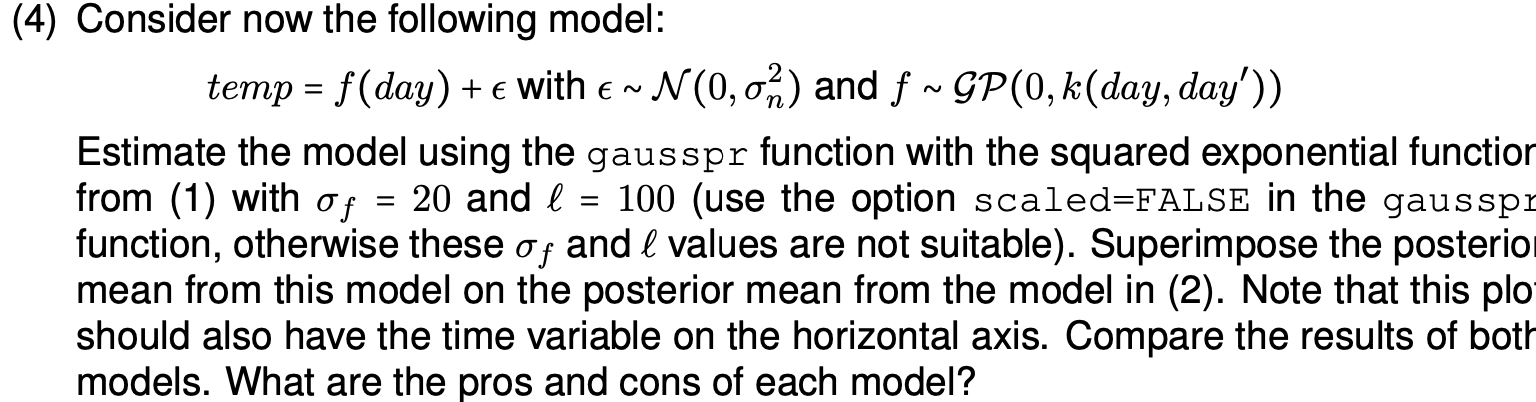
\includegraphics{images/Screenshot 2024-10-13 at 18.38.30.png}

\begin{Shaded}
\begin{Highlighting}[]
\NormalTok{SEK }\OtherTok{\textless{}{-}} \FunctionTok{nestedSEK}\NormalTok{(}\AttributeTok{sigmaF =} \DecValTok{20}\NormalTok{, }\AttributeTok{l =} \DecValTok{100}\NormalTok{)}

\NormalTok{modelGP }\OtherTok{\textless{}{-}} \FunctionTok{gausspr}\NormalTok{(trainData}\SpecialCharTok{$}\NormalTok{day, trainData}\SpecialCharTok{$}\NormalTok{temp, }\AttributeTok{scaled =} \ConstantTok{FALSE}\NormalTok{, }\AttributeTok{kernel =}\NormalTok{ SEK, }\AttributeTok{var =}\NormalTok{ sigmaNoise}\SpecialCharTok{\^{}}\DecValTok{2}\NormalTok{)}

\NormalTok{posteriorMeanDay }\OtherTok{\textless{}{-}} \FunctionTok{predict}\NormalTok{(modelGP)}


\FunctionTok{plot}\NormalTok{(}\AttributeTok{x=}\NormalTok{ trainData}\SpecialCharTok{$}\NormalTok{time, }\AttributeTok{y =}\NormalTok{ trainData}\SpecialCharTok{$}\NormalTok{temp,}
     \AttributeTok{xlab =} \StringTok{"time"}\NormalTok{, }\AttributeTok{ylab =} \StringTok{"temp"}\NormalTok{, }\AttributeTok{main =} \StringTok{"Temperature predictions"}\NormalTok{, }\AttributeTok{lwd =} \FloatTok{1.5}\NormalTok{)}
\FunctionTok{lines}\NormalTok{(}\AttributeTok{x=}\NormalTok{trainData}\SpecialCharTok{$}\NormalTok{time, }\AttributeTok{y =}\NormalTok{ posteriorMeanTime, }\AttributeTok{col =} \StringTok{"red"}\NormalTok{, }\AttributeTok{lwd =} \DecValTok{2}\NormalTok{)}
\FunctionTok{lines}\NormalTok{(}\AttributeTok{x=}\NormalTok{trainData}\SpecialCharTok{$}\NormalTok{time, }\AttributeTok{y =}\NormalTok{ posteriorMeanDay, }\AttributeTok{col =} \StringTok{"blue"}\NormalTok{, }\AttributeTok{lwd =} \DecValTok{2}\NormalTok{)}
\FunctionTok{legend}\NormalTok{(}\StringTok{"bottomright"}\NormalTok{, }\AttributeTok{legend=}\FunctionTok{c}\NormalTok{(}\StringTok{"Data"}\NormalTok{, }\StringTok{"Prediction Time"}\NormalTok{, }\StringTok{"Prediction Day"}\NormalTok{), }\AttributeTok{pch=}\FunctionTok{c}\NormalTok{(}\DecValTok{1}\NormalTok{, }\ConstantTok{NA}\NormalTok{, }\ConstantTok{NA}\NormalTok{), }\AttributeTok{lty=}\FunctionTok{c}\NormalTok{(}\ConstantTok{NA}\NormalTok{, }\DecValTok{1}\NormalTok{, }\DecValTok{1}\NormalTok{), }\AttributeTok{lwd=}\FunctionTok{c}\NormalTok{(}\ConstantTok{NA}\NormalTok{, }\DecValTok{2}\NormalTok{, }\DecValTok{2}\NormalTok{), }\AttributeTok{col=}\FunctionTok{c}\NormalTok{(}\StringTok{"black"}\NormalTok{, }\StringTok{"red"}\NormalTok{, }\StringTok{"blue"}\NormalTok{))}
\end{Highlighting}
\end{Shaded}

\includegraphics{lab4_files/figure-latex/unnamed-chunk-11-1.pdf}

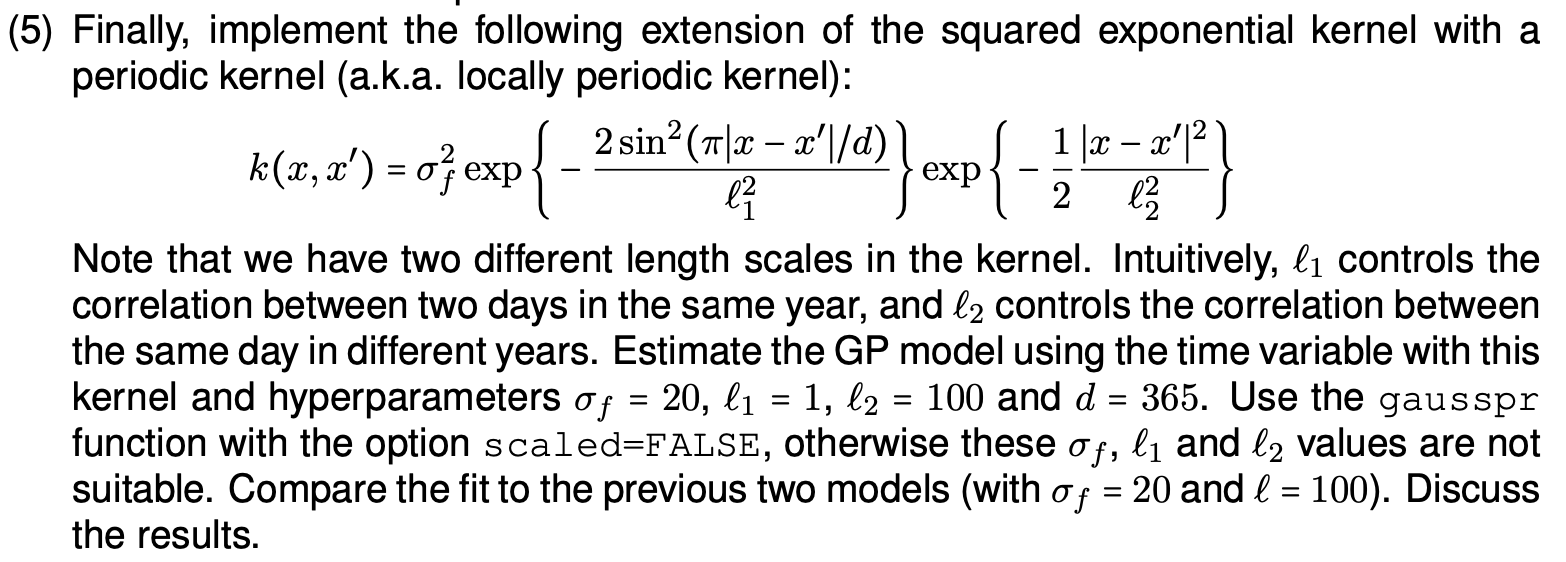
\includegraphics{images/Screenshot 2024-10-13 at 19.08.37.png}

\begin{Shaded}
\begin{Highlighting}[]
\NormalTok{periodicKernel }\OtherTok{\textless{}{-}} \ControlFlowTok{function}\NormalTok{(x, xstar, }\AttributeTok{sigmaF =} \DecValTok{20}\NormalTok{,}\AttributeTok{l1 =}\DecValTok{1}\NormalTok{, }\AttributeTok{l2 =} \DecValTok{100}\NormalTok{, }\AttributeTok{d=}\DecValTok{365}\NormalTok{)\{}
\NormalTok{  absDiff }\OtherTok{\textless{}{-}} \FunctionTok{abs}\NormalTok{(x}\SpecialCharTok{{-}}\NormalTok{xstar)}
  \FunctionTok{return}\NormalTok{(sigmaF}\SpecialCharTok{\^{}}\DecValTok{2}\SpecialCharTok{*}\FunctionTok{exp}\NormalTok{(}\SpecialCharTok{{-}}\DecValTok{2}\SpecialCharTok{*}\FunctionTok{sin}\NormalTok{(pi}\SpecialCharTok{*}\NormalTok{absDiff}\SpecialCharTok{/}\NormalTok{d)}\SpecialCharTok{\^{}}\DecValTok{2}\SpecialCharTok{/}\NormalTok{l1}\SpecialCharTok{\^{}}\DecValTok{2}\NormalTok{)}\SpecialCharTok{*}\FunctionTok{exp}\NormalTok{(}\SpecialCharTok{{-}}\DecValTok{1}\SpecialCharTok{/}\DecValTok{2}\SpecialCharTok{*}\NormalTok{absDiff}\SpecialCharTok{\^{}}\DecValTok{2}\SpecialCharTok{/}\NormalTok{l2))}
\NormalTok{\}}
\FunctionTok{class}\NormalTok{(periodicKernel) }\OtherTok{\textless{}{-}} \StringTok{\textquotesingle{}kernel\textquotesingle{}}


\NormalTok{modelGP }\OtherTok{\textless{}{-}} \FunctionTok{gausspr}\NormalTok{(trainData}\SpecialCharTok{$}\NormalTok{time, trainData}\SpecialCharTok{$}\NormalTok{temp, }\AttributeTok{scaled =} \ConstantTok{FALSE}\NormalTok{, }\AttributeTok{kernel =}\NormalTok{ periodicKernel, }\AttributeTok{var =}\NormalTok{ sigmaNoise}\SpecialCharTok{\^{}}\DecValTok{2}\NormalTok{)}


\NormalTok{posteriorMeanPeriodic }\OtherTok{\textless{}{-}} \FunctionTok{predict}\NormalTok{(modelGP)}


\FunctionTok{plot}\NormalTok{(}\AttributeTok{x=}\NormalTok{ trainData}\SpecialCharTok{$}\NormalTok{time, }\AttributeTok{y =}\NormalTok{ trainData}\SpecialCharTok{$}\NormalTok{temp,}
     \AttributeTok{xlab =} \StringTok{"time"}\NormalTok{, }\AttributeTok{ylab =} \StringTok{"temp"}\NormalTok{, }\AttributeTok{main =} \StringTok{"Temperature predictions"}\NormalTok{, }\AttributeTok{lwd =} \FloatTok{1.5}\NormalTok{)}
\FunctionTok{lines}\NormalTok{(}\AttributeTok{x=}\NormalTok{trainData}\SpecialCharTok{$}\NormalTok{time, }\AttributeTok{y =}\NormalTok{ posteriorMeanPeriodic, }\AttributeTok{col =} \StringTok{"green"}\NormalTok{, }\AttributeTok{lwd =} \DecValTok{2}\NormalTok{)}
\FunctionTok{lines}\NormalTok{(}\AttributeTok{x=}\NormalTok{trainData}\SpecialCharTok{$}\NormalTok{time, }\AttributeTok{y =}\NormalTok{ posteriorMeanTime, }\AttributeTok{col =} \StringTok{"red"}\NormalTok{, }\AttributeTok{lwd =} \DecValTok{2}\NormalTok{)}
\FunctionTok{lines}\NormalTok{(}\AttributeTok{x=}\NormalTok{trainData}\SpecialCharTok{$}\NormalTok{time, }\AttributeTok{y =}\NormalTok{ posteriorMeanDay, }\AttributeTok{col =} \StringTok{"blue"}\NormalTok{, }\AttributeTok{lwd =} \DecValTok{2}\NormalTok{)}
\FunctionTok{legend}\NormalTok{(}\StringTok{"bottomright"}\NormalTok{, }\AttributeTok{legend=}\FunctionTok{c}\NormalTok{(}\StringTok{"Data"}\NormalTok{, }\StringTok{"Prediction Time"}\NormalTok{, }\StringTok{"Prediction Day"}\NormalTok{, }\StringTok{"Prediction Periodic"}\NormalTok{), }\AttributeTok{pch=}\FunctionTok{c}\NormalTok{(}\DecValTok{1}\NormalTok{, }\ConstantTok{NA}\NormalTok{, }\ConstantTok{NA}\NormalTok{, }\ConstantTok{NA}\NormalTok{), }\AttributeTok{lty=}\FunctionTok{c}\NormalTok{(}\ConstantTok{NA}\NormalTok{, }\DecValTok{1}\NormalTok{, }\DecValTok{1}\NormalTok{, }\DecValTok{1}\NormalTok{), }\AttributeTok{lwd=}\FunctionTok{c}\NormalTok{(}\ConstantTok{NA}\NormalTok{, }\DecValTok{2}\NormalTok{, }\DecValTok{2}\NormalTok{, }\DecValTok{2}\NormalTok{), }\AttributeTok{col=}\FunctionTok{c}\NormalTok{(}\StringTok{"black"}\NormalTok{, }\StringTok{"red"}\NormalTok{, }\StringTok{"blue"}\NormalTok{, }\StringTok{"green"}\NormalTok{))}
\end{Highlighting}
\end{Shaded}

\includegraphics{lab4_files/figure-latex/unnamed-chunk-12-1.pdf}

\section{Part 2.3}\label{part-2.3}

\textbf{Import \& Data}

\begin{Shaded}
\begin{Highlighting}[]
\CommentTok{\#library(AtmRay)}

\CommentTok{\#install.packages("https://cran.r{-}project.org/src/contrib/Archive/AtmRay/AtmRay\_1.31.tar.gz", repos = NULL, type = "source")}

\FunctionTok{library}\NormalTok{(kernlab)}
\FunctionTok{library}\NormalTok{(AtmRay)}

\NormalTok{data }\OtherTok{\textless{}{-}} \FunctionTok{read.csv}\NormalTok{(}\StringTok{"https://github.com/STIMALiU/AdvMLCourse/raw/master/GaussianProcess/Code/banknoteFraud.csv"}\NormalTok{, }\AttributeTok{header=}\ConstantTok{FALSE}\NormalTok{, }\AttributeTok{sep=}\StringTok{","}\NormalTok{) }
\FunctionTok{names}\NormalTok{(data) }\OtherTok{\textless{}{-}} \FunctionTok{c}\NormalTok{(}\StringTok{"varWave"}\NormalTok{,}\StringTok{"skewWave"}\NormalTok{,}\StringTok{"kurtWave"}\NormalTok{,}\StringTok{"entropyWave"}\NormalTok{,}\StringTok{"fraud"}\NormalTok{) }
\NormalTok{data[,}\DecValTok{5}\NormalTok{] }\OtherTok{\textless{}{-}} \FunctionTok{as.factor}\NormalTok{(data[,}\DecValTok{5}\NormalTok{])}

\FunctionTok{set.seed}\NormalTok{(}\DecValTok{111}\NormalTok{)}
\NormalTok{SelectTraining }\OtherTok{\textless{}{-}} \FunctionTok{sample}\NormalTok{(}\DecValTok{1}\SpecialCharTok{:}\FunctionTok{dim}\NormalTok{(data)[}\DecValTok{1}\NormalTok{], }\AttributeTok{size =} \DecValTok{1000}\NormalTok{, }\AttributeTok{replace =} \ConstantTok{FALSE}\NormalTok{)}
\NormalTok{trainData }\OtherTok{\textless{}{-}}\NormalTok{ data[SelectTraining,]}
\NormalTok{testData }\OtherTok{\textless{}{-}}\NormalTok{ data[}\SpecialCharTok{{-}}\NormalTok{SelectTraining,]}

\CommentTok{\#accuracy function}
\NormalTok{accuracy }\OtherTok{\textless{}{-}} \ControlFlowTok{function}\NormalTok{(true, pred)\{}
  \FunctionTok{return}\NormalTok{(}\FunctionTok{mean}\NormalTok{(true }\SpecialCharTok{==}\NormalTok{ pred))}
\NormalTok{\}}
\end{Highlighting}
\end{Shaded}

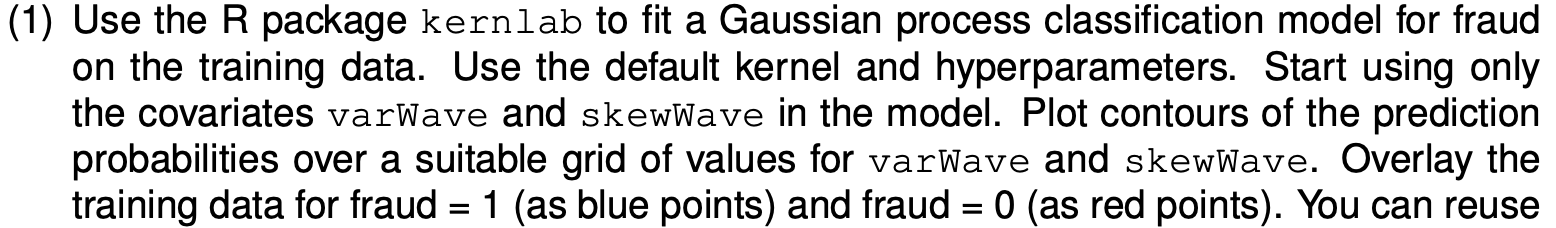
\includegraphics{images/Screenshot 2024-10-13 at 20.10.54.png}

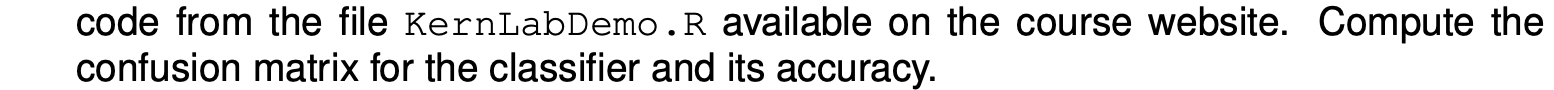
\includegraphics{images/Screenshot 2024-10-13 at 20.11.11.png}

\begin{Shaded}
\begin{Highlighting}[]
\NormalTok{GPfitFraud }\OtherTok{\textless{}{-}} \FunctionTok{gausspr}\NormalTok{(fraud }\SpecialCharTok{\textasciitilde{}}\NormalTok{ varWave }\SpecialCharTok{+}\NormalTok{ skewWave, }\AttributeTok{data=}\NormalTok{trainData)}
\end{Highlighting}
\end{Shaded}

\begin{verbatim}
## Using automatic sigma estimation (sigest) for RBF or laplace kernel
\end{verbatim}

\begin{Shaded}
\begin{Highlighting}[]
\NormalTok{predictionTrain }\OtherTok{\textless{}{-}} \FunctionTok{predict}\NormalTok{(GPfitFraud)}

\FunctionTok{table}\NormalTok{(trainData}\SpecialCharTok{$}\NormalTok{fraud, predictionTrain)}
\end{Highlighting}
\end{Shaded}

\begin{verbatim}
##    predictionTrain
##       0   1
##   0 503  41
##   1  18 438
\end{verbatim}

\begin{Shaded}
\begin{Highlighting}[]
\FunctionTok{accuracy}\NormalTok{(trainData}\SpecialCharTok{$}\NormalTok{fraud, predictionTrain)}
\end{Highlighting}
\end{Shaded}

\begin{verbatim}
## [1] 0.941
\end{verbatim}

\begin{Shaded}
\begin{Highlighting}[]
\CommentTok{\# class probabilities }
\NormalTok{probPreds }\OtherTok{\textless{}{-}} \FunctionTok{predict}\NormalTok{(GPfitFraud, }\AttributeTok{type=}\StringTok{"probabilities"}\NormalTok{)}
\NormalTok{x1 }\OtherTok{\textless{}{-}} \FunctionTok{seq}\NormalTok{(}\FunctionTok{min}\NormalTok{(trainData}\SpecialCharTok{$}\NormalTok{varWave),}\FunctionTok{max}\NormalTok{(trainData}\SpecialCharTok{$}\NormalTok{varWave),}\AttributeTok{length=}\DecValTok{100}\NormalTok{)}
\NormalTok{x2 }\OtherTok{\textless{}{-}} \FunctionTok{seq}\NormalTok{(}\FunctionTok{min}\NormalTok{(trainData}\SpecialCharTok{$}\NormalTok{skewWave),}\FunctionTok{max}\NormalTok{(trainData}\SpecialCharTok{$}\NormalTok{skewWave),}\AttributeTok{length=}\DecValTok{100}\NormalTok{)}
\NormalTok{gridPoints }\OtherTok{\textless{}{-}} \FunctionTok{meshgrid}\NormalTok{(x1, x2)}
\NormalTok{gridPoints }\OtherTok{\textless{}{-}} \FunctionTok{cbind}\NormalTok{(}\FunctionTok{c}\NormalTok{(gridPoints}\SpecialCharTok{$}\NormalTok{x), }\FunctionTok{c}\NormalTok{(gridPoints}\SpecialCharTok{$}\NormalTok{y))}

\NormalTok{gridPoints }\OtherTok{\textless{}{-}} \FunctionTok{data.frame}\NormalTok{(gridPoints)}
\FunctionTok{names}\NormalTok{(gridPoints) }\OtherTok{\textless{}{-}} \FunctionTok{names}\NormalTok{(trainData)[}\DecValTok{1}\SpecialCharTok{:}\DecValTok{2}\NormalTok{]}
\NormalTok{probPreds }\OtherTok{\textless{}{-}} \FunctionTok{predict}\NormalTok{(GPfitFraud, gridPoints, }\AttributeTok{type=}\StringTok{"probabilities"}\NormalTok{)}

\CommentTok{\# Plotting for Prob(setosa)}
\FunctionTok{contour}\NormalTok{(x1,x2,}\FunctionTok{matrix}\NormalTok{(probPreds[,}\DecValTok{1}\NormalTok{],}\DecValTok{100}\NormalTok{,}\AttributeTok{byrow =} \ConstantTok{TRUE}\NormalTok{), }\DecValTok{20}\NormalTok{, }\AttributeTok{xlab =} \StringTok{"varSkew"}\NormalTok{, }\AttributeTok{ylab =} \StringTok{"skewWave"}\NormalTok{, }\AttributeTok{main =} \StringTok{\textquotesingle{}Prob(fraud), fraud is red\textquotesingle{}}\NormalTok{)}
\FunctionTok{points}\NormalTok{(trainData[trainData}\SpecialCharTok{$}\NormalTok{fraud}\SpecialCharTok{==}\DecValTok{1}\NormalTok{,}\DecValTok{1}\NormalTok{],trainData[trainData}\SpecialCharTok{$}\NormalTok{fraud}\SpecialCharTok{==}\DecValTok{1}\NormalTok{,}\DecValTok{2}\NormalTok{],}\AttributeTok{col=}\StringTok{"red"}\NormalTok{)}
\FunctionTok{points}\NormalTok{(trainData[trainData}\SpecialCharTok{$}\NormalTok{fraud}\SpecialCharTok{==}\DecValTok{0}\NormalTok{,}\DecValTok{1}\NormalTok{],trainData[trainData}\SpecialCharTok{$}\NormalTok{fraud}\SpecialCharTok{==}\DecValTok{0}\NormalTok{,}\DecValTok{2}\NormalTok{],}\AttributeTok{col=}\StringTok{"blue"}\NormalTok{)}
\end{Highlighting}
\end{Shaded}

\includegraphics{lab4_files/figure-latex/unnamed-chunk-14-1.pdf}

\hfill\break

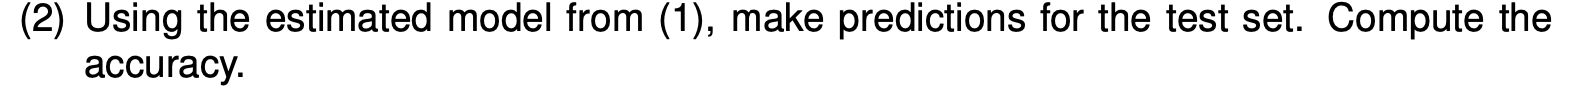
\includegraphics{images/Screenshot 2024-10-13 at 20.11.27.png}

\begin{Shaded}
\begin{Highlighting}[]
\NormalTok{predictionTest }\OtherTok{\textless{}{-}} \FunctionTok{predict}\NormalTok{(GPfitFraud, testData[,}\FunctionTok{c}\NormalTok{(}\DecValTok{1}\NormalTok{,}\DecValTok{2}\NormalTok{)])}

\FunctionTok{accuracy}\NormalTok{(testData}\SpecialCharTok{$}\NormalTok{fraud, predictionTest)}
\end{Highlighting}
\end{Shaded}

\begin{verbatim}
## [1] 0.9247312
\end{verbatim}

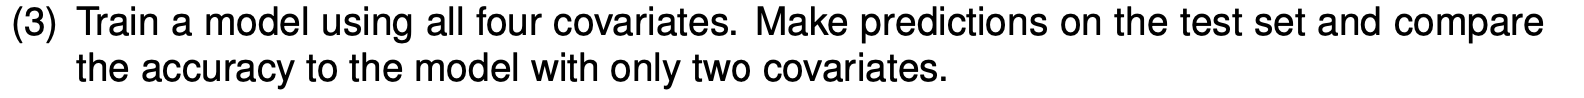
\includegraphics{images/Screenshot 2024-10-13 at 20.11.36.png}\\

\begin{Shaded}
\begin{Highlighting}[]
\NormalTok{GPfitFraud4 }\OtherTok{\textless{}{-}} \FunctionTok{gausspr}\NormalTok{(fraud }\SpecialCharTok{\textasciitilde{}}\NormalTok{ ., }\AttributeTok{data=}\NormalTok{trainData)}
\end{Highlighting}
\end{Shaded}

\begin{verbatim}
## Using automatic sigma estimation (sigest) for RBF or laplace kernel
\end{verbatim}

\begin{Shaded}
\begin{Highlighting}[]
\NormalTok{prediction4 }\OtherTok{\textless{}{-}} \FunctionTok{predict}\NormalTok{(GPfitFraud4, testData[,}\SpecialCharTok{{-}}\DecValTok{5}\NormalTok{])}
\FunctionTok{accuracy}\NormalTok{(testData}\SpecialCharTok{$}\NormalTok{fraud, prediction4)}
\end{Highlighting}
\end{Shaded}

\begin{verbatim}
## [1] 0.9946237
\end{verbatim}

\end{document}
